\documentclass{acm_proc_article-sp}

\usepackage{graphicx}
\usepackage{bussproofs}
\usepackage{amssymb}
\usepackage{amssymb}
\usepackage{listings}
\usepackage{color}
\usepackage{caption}

\lstset{numbers=left, numberstyle=\small, numbersep=8pt, frame = single, language=Java, framexleftmargin=15pt}

\DeclareCaptionFont{white}{\color{white}}
\DeclareCaptionFormat{listing}{\colorbox{gray}{\parbox{\textwidth}{#1#2#3}}}
\captionsetup[lstlisting]{format=listing,labelfont=white,textfont=white}

\begin{document}

\title{Distributed Intents for the Android platform}

\author{
Kristopher Micinski\\
       \email{micinski@cs.umd.edu}
\and
Brianna Ren\\
       \email{bren@cs.umd.edu}
}

\maketitle

\begin{abstract}
  The Android platform exhibits a service oriented architecture where
  apps can interact with each other through message passing.  These
  messages --- called intents --- use late binding to allow any number
  of apps to handle them, based on a filter which is used to decide
  which app will respond to the intent.  This gives rise to a
  programming style based on late binding.  We formalize these
  intents, and present inter device intents, allowing multiple devices
  to communicate and accomplish a task, even if the tools to
  accomplish the task do not exist (together) on any single device.
  We have a working implementation based on a combination of an
  Android library and a Rails web service (which does intent routing
  for us).  To demonstrate our system --- and as a case study in
  distributed programming and collective computation --- we design a
  sample app which showcases the use of our library and associated web
  service.
\end{abstract}

\section{Introduction}
Android applications exhibit a novel programming model: a service
oriented architecture with message passing between applications to
allow cooperation.  As an example, we might have an application which
allows a user to take a picture, manipulate it with a photo editor (to
remove red eye, for example), and then send it to their friends via
email.  The messages sent between applications are called Intents, and
form the basis for service oriented communication.  This is a great
vision: it allows apps to be written extremely concisely and with
minimal code.

Our goal is to make Android programs act like modules of a program:
exporting an interface with which other programs can interact.  Each
app has specialized functionality, for example, an email app may store
certain preferences about the user (their main email address).  But it
is helpful for these apps to interact (such as using the preferred
email app to back up information), because the user will be used to
their preferred email application to back up their contacts (for
example).

In this paper we present:

\begin{itemize}
\item A formalization of intents, and the Android activity stack.
  This allows precise reasoning about how intents will be handled and
  allows an interpretation of exactly what in intent \emph{is}.

\item A proposal for distributed programming with intents, where the
  intent names a set of constraints (in accordance with our formalism)
  used for finding which applications can handle those intents.

\item A sample implementation of both a library for manipulating and
  programming with intents, and example application using our approach
  and showing its correctness.

\end{itemize}

\section{Intents in Android}
\label{sec:intent-overview}

Intents in Android are lightweight messages across sent process
boundaries used for a variety of purposes: they are the main
interprocess communication primitive in the system. Figure
~\ref{fig:intent-example} gives an example of an Intent as it is used
in the Android system.  An intent object is a late bound message
asking the system perform some work on the Application's behalf.
After the work is performed, the system can call back into the
application with a result, after which the system can do more work.

Intents in Android allow the following:

\begin{itemize}
\item Launch a new screen to perform an action.
\item Send a broadcast to a background service.
\item Start a background service.
\end{itemize}

Essentially, some intents require user interaction, while others do
not.  We classify intents in a number of different categories, which
will be important for our later discussion of interapp and
inter-device intents.

\begin{itemize}
\item Interaction based, versus background.
\item Stateful, versus stateless.
\item Persistent, versus atomic.
\end{itemize}

We give several examples to motivate this classification.  Some
intents are messages to the system that request an app to be started
so that the user may enter data, then go back to the original app
after accepting some input.  An example of these are the camera app
(take a picture) or contacts app (choosing a contact to which an email
will be sent).  Some intents generate stateful actions: they change
the state of the current device.  An example of this type of intent is
a request to change a contact's phone number.  This would affect the
state of the current device.  By contrast, choosing a contact does not
manipulate the state of the current device.  Finally, by a persistent
intent, we mean that which starts a persistent action, such a long
running service to send weather information to the user.  Again,
picking a contact would be an atomic operation.

\subsection{Current Intent System}

Applications currently use intents to send lightweight messages to
other processes, for sharing data, starting services, and querying the
user to perform certain UI interactions.  To send an intent, a
programmer constructs a new \texttt{Intent} object specifying certain
fields.  After constructing an intent, the programmer sends the intent
to the system via calling one of a number of service methods: 
\begin{itemize}
\item \texttt{startActivity} --- Prompt the user for UI
  interaction. (e.g., choose a file.)
\item \texttt{broadcastIntent} --- Send a message to another program
  on the device.
\item \texttt{startService} --- Start (or send a message to) a
  background service with which the current program will interact.
\end{itemize}
Each of these methods accepts an intent object saying which program
should receive the message.  Because Android programs can die at any
time (and be restarted), receiving a message from another program
wakes up the receiver and places it back at a running state.

The Android platform and documentation makes a distinction between
\emph{explicit} and \emph{implicit} intents.  An explicit intent is an
intent which names a package (specific Java code) which should handle
the intent.  An example of this kind of intent is requesting the
system to scan a QR code, using a specific QR code scanner, using a
specific scanner installed on many systems.
Figure~\ref{fig:qr-scanning-intent}.  (Examples in this section are
examples given in a Google Android developers blog post exhibiting the
use of intents \ref{android:intentblog}.)

\begin{figure}
  \caption{QR Scannig Intent}
  \label{fig:qr-scanning-intent}
  \begin{lstlisting}
Intent intent = new Intent(
  ``com.google.zxing.client.android.SCAN'');
// This flag clears the called app from 
// the activity stack
intent.addFlags(
 Intent.FLAG_ACTIVITY_CLEAR_WHEN_TASK_RESET);
// Set Scan mode
intent.putExtra(``SCAN_MODE'', 
  ``QR_CODE_MODE'');
startActivityForResult(intent, 0);
  \end{lstlisting}
\end{figure}

An implicit intent fills out other fields of the intent
and allows the system package manager free to choose the best program
to handle the intent.  An example of this kind of functionality might
be sending a picture.  For this, the user would take a picture, the
camera app constructs an intent specifiying the name of the picture
and its MIME type (a jpeg image, for example) and then specify the
\texttt{ACTION\_SEND} action (specifying the action to be performed).  The
system would then see there were multiple programs capable of handling
the intent, among them the email app and the bluetooth app.
Figure~\ref{fig:share-intent} 
shows an example of this kind of intent
being sent to the system, we highlight it because it is similar to
the intent that we construct for our email in our case study
(Section~\ref{section:case-study}).

\begin{figure}
  \caption{Share Intent}
  \label{fig:share-intent}
  \begin{lstlisting}
// Construct the skeleton of the intent
Intent intent=
  new Intent(Intent.ACTION_SEND);
intent.setType(``text/plain'');
intent.addFlags(
  FLAG_ACTIVITY_CLEAR_WHEN_TASK_RESET);

// Add data to the intent, the receiving
// app will decide what to do with it.
intent.putExtra(Intent.EXTRA_SUBJECT, 
  ``Some Subject Line'');
intent.putExtra(Intent.EXTRA_TEXT,
 ``Body of the message, woot!'');

// Send the intent to the system and
// start a new UI to send the message
startActivityForResult(intent);
\end{lstlisting}
\end{figure}

%\section{Higher Order Intents}
% \section{Model of Intents}
% \section{Android Scheme}
% In this section we present Android scheme, a small language which we
% have invented to enable scripting with (and demonstrate the power of)
% android intents.  A user (who wants to write Android apps, out of
% existing Android components) will write their app using Android
% scheme, and then pass those programs to the Android scheme
% interpreter, running on a device (this is a standard app, with some
% boilerplate code).
% Each intent is handled \emph{within} its handling app, and only the
% result of the computation leaves the intent, but this is no problem:
% we can simply write programs in Android scheme, and then have the
% indivual intents call back to the interpreter when they finish, using
% a continuation based style.  Android already encourages this
% programming style, as when intents finish the can start new intents by
% simply passing them to the system.

\section{Formalization of Intents}

The Android system resolves intents sent to other processes by using
map defined in the system.  When an application is installed, it also
carries a manifest file specifying all of the components of the
application, along with various other metadata (for security, icons,
etc...).  Upon installation, the system package manager registers an
app.  When an intent is used (or queried) the package manager simply
uses this mapping to find which components can handle the intent.  Our
formalism of intents seeks to capture this notion.

To model intents, we use a set of constraints.  Each intent handler in
the Android platform handles one of these constraints by providing a
guarantee that the intent can be handled.  We do not concentrate too
particularly on a specific formalism from logic, because the intent
system can be encoded in any first order logic.  Particularly we
consider an intent $\mathcal{I}$ as a tuple, along with a formula
$\mathcal{I}_\phi$.  We assume that $\phi$ specifies certain relations
used to \emph{match} the intent with a handler: any handler which
solves (logically) the intent can execute code based on the arguments
in $\mathcal{I}$.  (In our implementation we use equality over
predicates with variadic string arguments, though other formulations
are possible.)  For our purposes, we consider that constraint is a
conjunction of literals, each consisting of predicates over
universally quantified variables.  We could imagine a more complex
system for specifying intents, for example using first order logic.
We choose with a subset of first order logic because we did not find
any real examples in the Android framework (that were not fabricated
by us) that necessitated their incorporation: doing so simply made the
system more complicated.

An intent handler registers to receive intents by specifying which
intents they can reliably handle.  We view as an intent handler as a
function $f$, which accepts an intent $\mathcal{I}$ as input, along
with a provided matching formula: $\phi$.  We consider the system to
have a large set of intents, $\Gamma$.  To decide whether an intent
can be handled or not, we attempt to --- for each $\phi \in \Gamma$,
solve the formula, $\phi \implies \mathcal{I}_\phi$.  If any handler
solves the formula, it can handle the intent.  In the Android
framework, there are situations in which multiple handlers can execute
an intent, Figure~\ref{fig:multiple-intents} shows an example where

\paragraph*{Example: sending email through a client} 
We might model an intent for an email client by giving the email
subject, sendee, and text, along with a predicate \texttt{mimeType},
which specified the mime type used.  In this case, the intent
specifies a formula such as the following: \texttt{sendee =
  email@example.com} $\land$ \texttt{body = some text...} $\land$
$Handles($\texttt{someFormat}$)$.  In this example, we used the
$Handles$ predicate.  In general the set of predicates is unbounded,
we do not provide any infrastructure to make the predicates unique.
In particular, we could also use a hierarchical namespace of
predicates prefixed by the application package: this is simply naming
convention.

\paragraph*{Modeling the Android system intent}\label{section:intents-model}
All intents seen in the Android system match our formalism, we
investigted the implementation of the Android \texttt{PackageManager}
\ref{android:package-manager}.  We also found that intents are matched
only up to certain number of parameters, in particular only a few
fields are considered in some situations (in the case of a
\texttt{PendingIntent}.  We can handle all of the standard Android
intents (included in the standard apps that come preinstalled on the
device) using the formalism given in this section.

\begin{figure}[t]
  \centering
    \includegraphics[width=.3\textwidth]{sharing}
    \caption{When the system cannot fully resolve an intent, it is
      possible that there will be more than one process which can
      handle the intent.  In our model we view this as a nonempty
      handler set.}
\end{figure}

\section{Inter-Device Intents}

As part of our project, we considered the possibility of inter device
intents.  While the vanilla Android programming model allows sending
intents to other programs on the same device, there are occasions when
a user may not have the program required to handle the intent on their
device, but another device may have the intent.  We present a solution
to allow a set of devices to carry on a computation with other users
helping, by having their device receive intents and doing the required
work, then sending the required result back to the application.  This
has numerous benefits:

\begin{itemize}
\item Allows expressive communication patterns to be written at the
  application layer without complicated libraries to handle inter
  device communication.
\item Sharing code on other devices: if code for one intent
  can be handled by another device then any set of devices can
  effectively share capabilities across a network.
\end{itemize}

\paragraph*{Eligible Intents for Inter Device Communication:}

Unfortunately not all intents can be sent to other devices, because
only a subset of the intents make sense to be executed remotely.  For
example, if an app wants a file to be picked, it cannot send the file
picker intent to a remote device because it wouldn't make sense for
another user to select a color on behalf of a remote app.  The most
appropriate intents are background, stateless, and atomic intents,
such as those for printing a document.

Android already includes this class of intents as (roughly) the
broadcast intents, sent to other programs on the system, send via the
\texttt{broadcastIntent}.  In fact, this is the only type of intent we
consider in this prototype implementation: providing a subset of the
functionality that exists on Android today.

\paragraph*{Prototype Intent System}

To expand the current viewpoint of intents, we use our formalization
of intents as constraints and take this as the basis for an inter
device programming model.  There are a number of factors to consider,
but in our prototype implementation we simply want to have a simple
interface (to the programmer) that looks like the standard intent
interface.  We want to be able to define new intents on the fly and
set them up in the network for use by other devices.  To deliver
intents between devices, we need some mechanism.  While there are a
number of options (an ad hoc network, epidimic routing protocols,
etc...) this is not the focus of our project: we simply want to focus
on a framework which showcases the uses of distributed programming.
Because of this, we have chosen to use a web service along with Java
library (which communicates with the web service) which programmers
use.

We wish to emphasize that --- even though this system uses a web
service for a backend --- this could be changed without affecting the
view seen by the programmer.  The programmer would simply use a
library implementing the system having the same signature but using a
different routing algorithm.  (Our library currently provides no
gaurentees to the programmer on routing of messages between devices,
except timeouts, which are being added as current work.)

\section{The Web Service}\label{section:webservice}


In our project, we set up a RESTful web service to route intents between Android phones, so that communication can happen across the network.  The intent interface in our implementation talks to this service using standard HTTP communication.  We chose to set up the web service using Ruby on Rails (often shortened to Rails), a popular web application framework for the Ruby programming language with REST support.   In particular, our web service uses the Google Cloud Messaging (GCM) service for Android to respond to the devices.  GCM is a new technology released in June 2012 and is a free service that allows our web server to send lightweight messages to Android phones.  In our service, GCM is used as a simple protocol for sending messages for registered phones, in addition to allowing the web service to tell the Android phone that they have a new request or response.

Our web service stores information in two databases: a device registration database and an intent request database.


The first is a simple database that stores information about registered phones.  It stores two fields: 

 \begin{enumerate}
 \item device id - a constant id that uniquely identifies the device.
 \item device registration id - a registration id with GCM.
 \end{enumerate}

The main web service database stores information about each intent request, which includes:

\begin{enumerate}
\item Requester device id
\item Requester device registration id
\item Intent program (JSON string)
\item Output for successful completion
\item Error message for failure
\item Status (active / success / error)
\item Number of remote phones available to run the intent program
\item Number of errors received from remote phones for running the intent program
\end{enumerate}

Here we show how an intent request works with our web service.

\begin{enumerate}
\item Various Android phones register with our web service as available phones that can run intent programs.  

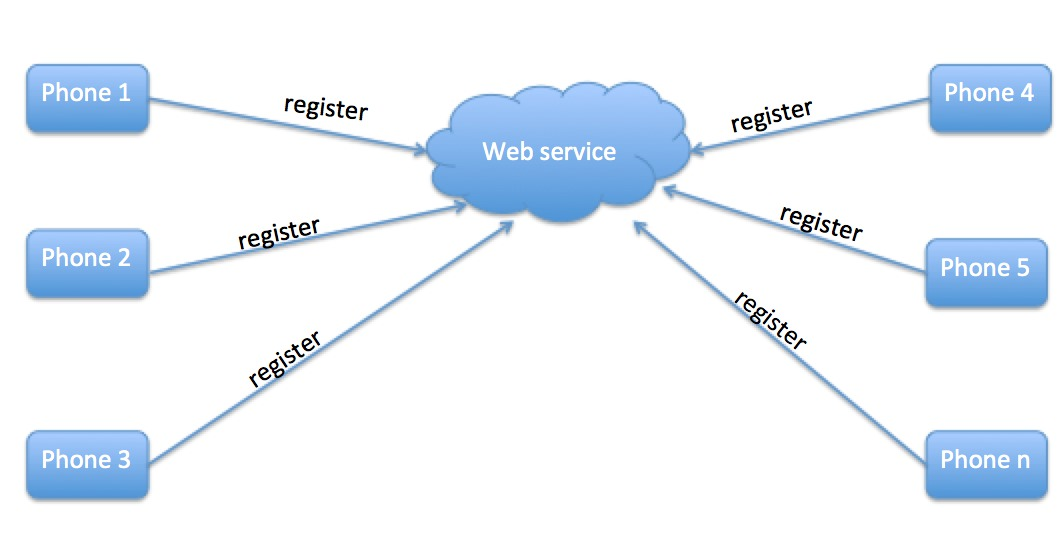
\includegraphics[scale=0.45]{s1.jpg}

\item An Android phone sends an intent request to our web service

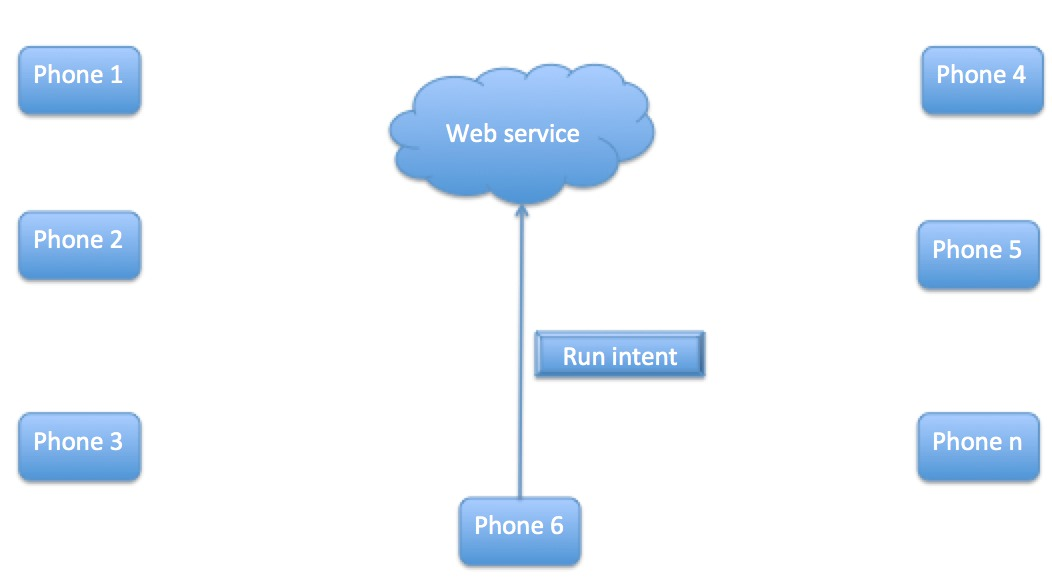
\includegraphics[scale=0.45]{s2.jpg}

\item  When an intent request is issued to our web service, the service will indirectly forward this request to all phones stored in our database, except the requester.  The intent is stored as a JSON string. Since the web service cannot talk to any phone directly, the web service first sends the intent to the Google Cloud Messaging service, which then forwards the request to the individual remote phones. 

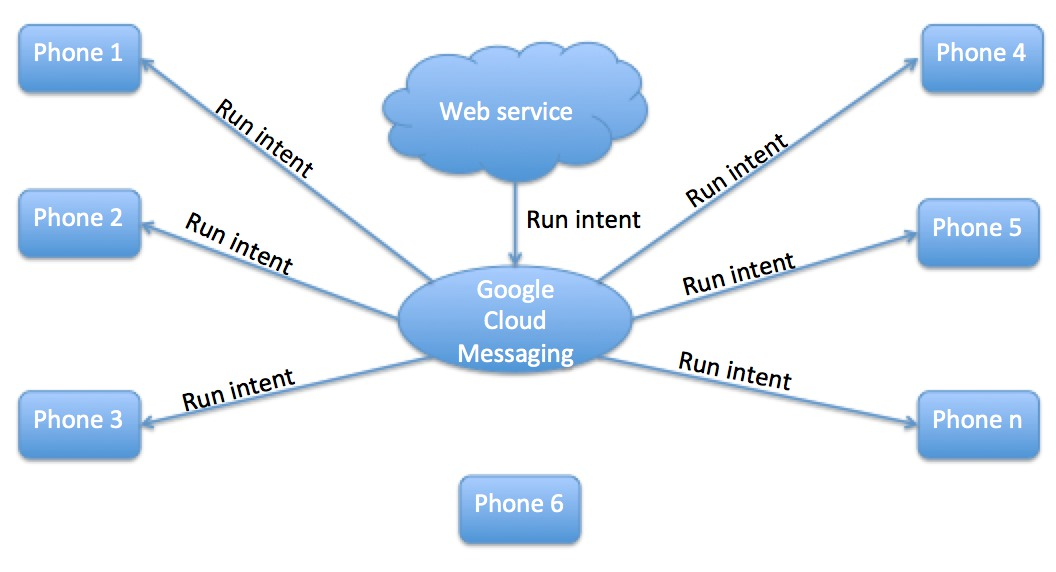
\includegraphics[scale=0.45]{s3.jpg}

\item Each remote phone will execute the intent when possible, and will directly contact our web service to inform us that it has finished the job.  The termination of executing an intent program on a remote phone indicates two distinct types of results: successful completion and failure.  Failure may involve errors like hardware problems.   If the job was successfully completed, then the web service will be informed of the success and the output.  If the job failed, then the web service will be informed of the failure along with the error message.

When the web service receives the first successful execution completion notification, it will send the output back to the requester through GCM. 

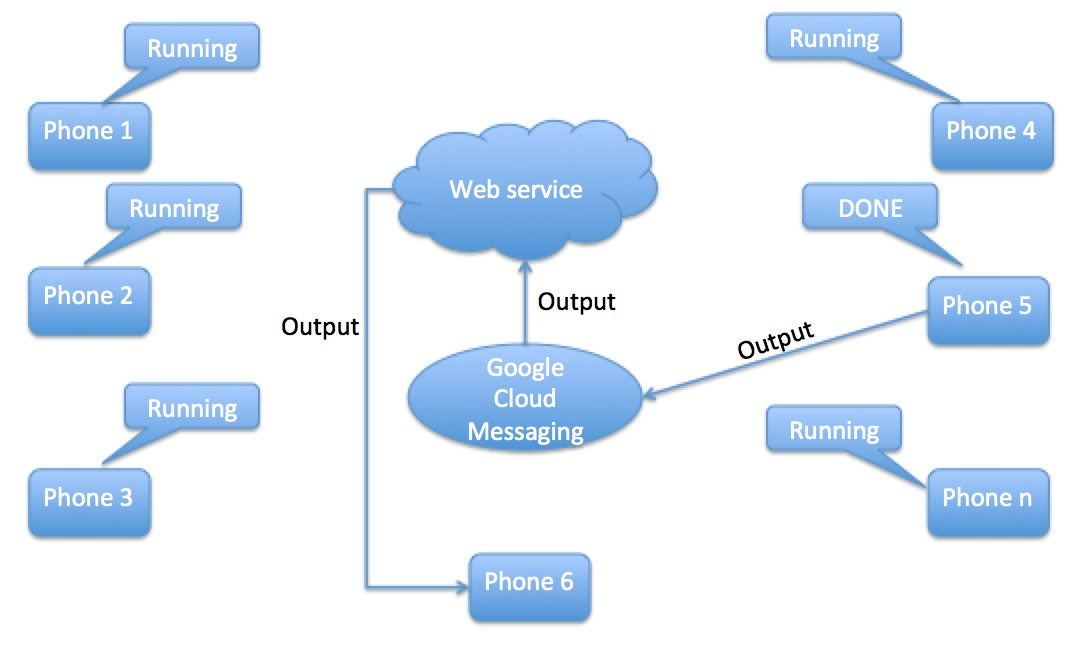
\includegraphics[scale=0.45]{s4a.jpg}

If all remote phones report back that the execution failed, then we send this result along with the error message back to the requester.

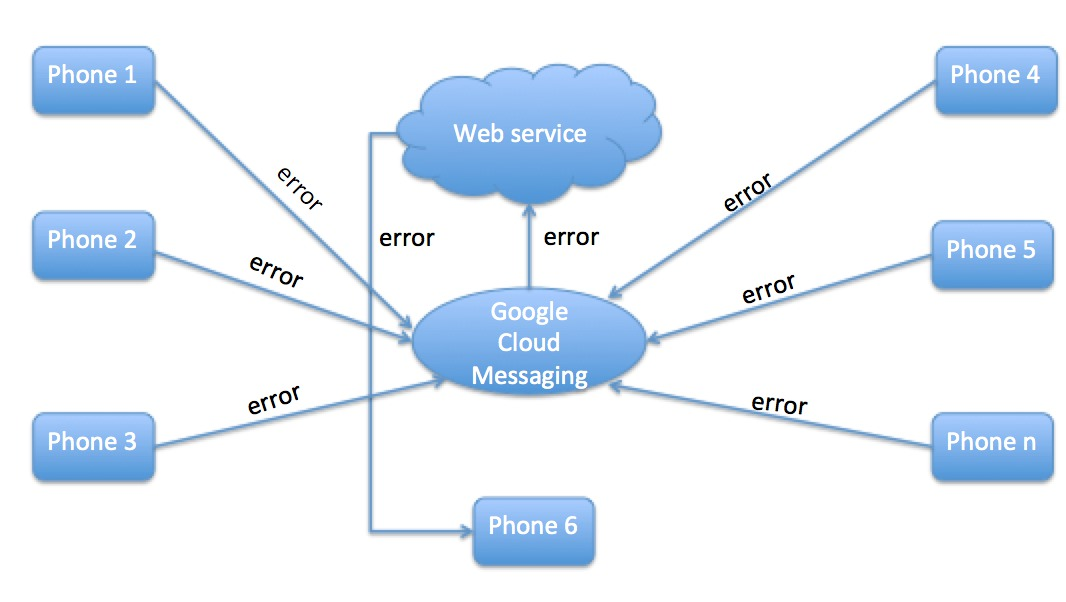
\includegraphics[scale=0.45]{s4b.jpg}

However, suppose there are n remote phones and the first n - 1 executions resulted in failure, but the last execution results in a success.  In this special case we will only report the successful execution with the output to the requester.

\end{enumerate}

In Rails, a Controller receives a request and produces the appropriate output. 
The main controller in our web service is the Rails intent request controller. 
We have included the key parts of the source code for this controller in the 
appendix with comments.


\section{The Java library}

We have implemented our remote intent formalism as a Java library
which can be linked in to Android programs.  It presents a simple
programming interface for defining and executing remote intents (that
can run locally if the programs are available).  The library interacts
with our webservice described in Section~\ref{section:webservice} to
route and deliver intents.  An example use 

\paragraph{The Broadcast Receiver}
To receive intents from other devices, we use a background service
which listens to network calls from the Google Cloud Messsaging
service.  Upon receiving an intent (sent from another device), our
background service will check the device for any registered receiver
which can handle the intent.

\paragraph{Representing Constraint Sets}

In our model of intents (Section~\ref{section:intents-model}) we view
intents as sets of constraints.  In our prototype implementation, we
model intents as sets of constraints on strings.  Our implementation
provides a set of classes
(\texttt{org.umd.mobileintents.ConstraintSet} and a few other related
classes) that allow constraints to be represented in Java, and then
transformed to (and from) JSON (so that they may be transmitted across
the network).

When writing an appliation which uses the mobile intents library, it
must first register a set of constraints with the background service
running on the device.  In registering an intent, an intent handler
constructs a constraint set which it provides to the system and calls
\texttt{registerProvider} with the constraint as an argument.

\paragraph{Matching constraints on the client device}

Because we represent constraints as simply first order formulae, to
decide whether an individual constraint can be satisfied or not, we
use a simple unification based solving strategy in the background
service.  To do matching, our background service looks at all of the
registered intent providers and checks to see if any of them unify
(with respect to first order formulae) with the intent.  Since some of
the variables will be universally quantified this simply means looking
for how to fill in holes in quantifiers: a simple procedure
implemented by our \texttt{ConstraintSolver} class.

\subsection{Communicating with the Web Service} 

To communicate with the web service, we use a background Android
Service.  This is necessary because network communication cannot
happen on the main (UI) thread in Android programs.  Fortunately, this
is taken care of by a convenience class: \texttt{MobileIntentHelper}.
An application binds to the intent helper class when the application
loads, but the user can simply get a singleton of this class using a
\texttt{Context} object provided by the system.  The intent helper
then performs background communication using an \texttt{HttpClient} in
the background.

The web service could have many intents being sent at the same time
between devices.  Because of this, each intent is identified with a
unique intent ID.  After sending the intent to the web service, it
responds with an intent ID.  This is used so that the device and
service can both be confident that they are really talking about the
same intent (and is also important to keep of which device should be
sent the result of an individual intent).

\section{Case Study: Time Tracking App}
\label{section:case-study}

As a case study for our distributed intent infrastructure, we
implemented a time tracking app which allows backing up the time
tracking database to a remote email source using a broadcast intent.
We provide this program (and associated service) as a simple example
of using our remote intent library.  Our implementation consists of
two parts:

\begin{itemize}
\item The time tracking app, which allows the user to track their time
  and backup t he information to an email account.
\item A service which provides the email intent functionality.
\end{itemize}

The time tracking app is a fairly complete app that demonstrates many
features of the Android platform (so as to provide support that our
system works for real app).  It allows the user to navigate through
several screens to keep track of what they are doing at any given
time.  Because the user may want process their time data, they will
typically want to export the data to a computer for analysis.  To
export the data, we propose simply emailing the data to the user so
that they may retrieve it and perform analysis on it.  

Because sending email is a somewhat complicated procedure, potentially
requiring third party libraries, a simple way to send the email would
simply be sending it via an intent.  We could simply use the
\texttt{ACTION\_SEND} intent to send the data with an appropriate MIME
type, but this typically prompts the user for UI interaction.
Instead, we choose to broadcast the intent and handle it using a
broadcast receiver.

Our app uses our mobile intents library to send an email intent, but
there must be a registered app to receive the intent.  To give an
example of how to write a mobile intent, we also provide an
implementation of an email handling intent.  This is a separate app
which registers the email intent with the mobile intents router on the
device.

\subsection{Backup in the Time Tracker App}

Among the activities in our time tracker app, we have a screen which
backs up the user's log to email.  The simplest way to do this is with
the code to send an email to the client.  This is accomplished using
the standard Android \texttt{SEND} intent.  For completeness, we have
implemented this in our class and show it as an example
(Figure~\ref{fig:send-email-intent}).

\begin{figure*}
  \begin{lstlisting}
public void onClick(View v) {
  Intent i = new Intent(Intent.ACTION_SEND);
  i.setType(``message/rfc822'');
  i.putExtra(Intent.EXTRA_TEXT, csvExporter);
  i.putExtra(Intent.EXTRA_EMAIL, new String[]{mEmailAddress});
  i.putExtra(Intent.EXTRA_SUBJECT, mSubject);
      
  try {
        startActivity(Intent.createChooser(i, ``Send backup email''));
  } catch (android.content.ActivityNotFoundException ex) {
    Toast.makeText(MyActivity.this, ``There are no email clients installed.'',
    Toast.LENGTH_SHORT).show();
  }
}
  \end{lstlisting}
  \caption{Backing up the contents of the database to an email account
    using the normal Android platform, using a standard
    \texttt{ACTION\_SEND} intent to accomplish the task.}
  \label{fig:send-email-intent}

\end{figure*}

Of course the problem with the mobile intents library is that the code
might not exist on the device.  To use our mobile intents library, we
simply adapt the code in figure \ref{fig:send-email-intent} to use our
mobile intents library.  Note that our code uses our constraint
objects (which will be similarly mirrored in the provider app) and
also carries extras (used in Android to specify parameters for the
intent).  Because \texttt{startActivity} is a method of the
\texttt{Activity} class, we have to use an intent helper to send the
message: this is simply a singleton class obtained when the class is
created which allows sending messages to the service.  Upon receiving
a result from the receiver we check to see if there is an error: this
would indicate that no device was capable of handling the intent.
Although this code also performs complex network and stateful
interactions with our web service and the cloud, it is still very
simple for the programmer to write.

\begin{figure}[t]  
  \begin{lstlisting}
public void onClick(View v) {
  MobileIntent i = new MobileIntent();
  Constraint sendAction = 
  new PredicateConstraint(``action'', 
    new AtomConstraint(``send''));
  Constraint messageType = 
    new PredicateConstraint(``mimetype'', 
    new AtomConstraint(
    ``message/rfc822''));
  i.addConstraint(sendAction);
  i.addConstraint(messageType);
  i.putExtra(Intent.EXTRA_TEXT, csv);
  i.putExtra(Intent.EXTRA_EMAIL,
    new String[]{mEmailAddress});
  i.putExtra(Intent.EXTRA_SUBJECT, mSub);
  mIntentHelper.broadcastIntent(i);
}

public void onReceiveMobileIntentResult(
    MobileIntentResult r) {
  if (!r.success()) {
    Toast.makeText(MyActivity.this,
    ``No email clients installed.'',
      Toast.LENGTH_SHORT).show();
  }
}
\end{lstlisting}
\caption{A modified version of the code to use our mobile intents
  library.  All of the pieces match up with the previous code with
  slight cosmetic changes accomodating the new intent library.}
\label{fig:mobile-intents-email-example}
\end{figure}

\subsection{Email Intent Handler}

To handle email and demonstrate handling distributed intents, we
implement our email handler as a separate app which registers with the
mobile intent service.  The app --- upon starting --- constructs an
intent set (shown in Figure~\ref{fig:email-intent-provider}) and then
registers it with the mobile intents provider.  The intents provider
then inserts the constraint provider set into the local database of
the device so that it can route intents properly upon receiving them.

Sending email on a device is complex.  We used open source code given
on the internet (TODO: REF HERE) along with the javamail API to send
email.  To properly handle the intent, we first register the intent
with the background service on the phone by creating an intent handler
and sending it to the service.

Creating an intent handler involves creating an instance of the
\texttt{ConstraintSet} class and filling out the appropriate fields.
We then pass the \texttt{ConstraintSet} to a
\texttt{MobileIntentHelper} object, which will register the intent
with the service running on the device.  The \texttt{registerService}
method also takes a \texttt{PendingIntent} as a parameter, which
allows an intent to be executed at a later time.  This allows the user
to write a normal broadcast handler (as in the Android platform) but
use a standard intent for it.  A pending intent is simply an intent
that will be executed later.  The intent service takes this intent
helper and stores it until an intent is received.

In the Android system, registering a broadcast receiver happens by the
system before the app runs.  Unfortunately, in our library we have to
register the service the first time the app is run.  Because of this,
we generally write intent registration code in an application's
\texttt{onCreate} class (which will be run when the application
opens).  This introdues some minor overhead, but only a very small
amount: it is a consequence of implmenting our approach as a library
rather than at the system level (which would be able to register the
intent handler in the sytem package manager as usual.  We do so in our
first activity (screen) in our sample application, the first thing
that runs, we give an example of doing so in
Figure~\ref{fig:registration-code}.

When the service receives messages from the Google Cloud Messaging
service, they contain references to messages from the web service.
Because a request might be quite large (GCM messages can only hold 4
kilobytes of data) we simply pass a reference to an ID (stored in a
database on the service) in the GCM message.  Once the device receives
the message, it handles it approriately.  Currently, there are the
following handlers:

\begin{itemize}
\item Pending request --- Another device has sent an intent which
  should be downloaded and handled if possible.
\item Intent response --- After sending an intent, the service has
  responded (after collecting answers from other nodes) with an
  answer.
\end{itemize}

\begin{figure*}
\begin{lstlisting}
Intent emailIntent = new Intent();
emailIntent.setComponent(EmailReceiver.class);
PendingIntent emailBroadcast = getBroadcast(this, 0, emailIntent, 0);
Constraint sendAction = 
  new PredicateConstraint(``action'', new AtomConstraint(``send''));
Constraint messageType = 
  new PredicateConstraint(``mimetype'', new VariableConstraint(``x''));
ConstraintSet constraints = 
  new ConstraintSet(new Constraint[] { sendAction, messageType});
mIntentHelper.registerIntent(constraints, emailBroadcast);
\end{lstlisting}
\caption{Registering an intent with the mobile intent service.  This
  is similar to registering a broadcast receiver with the Android
  platform.  The programmer writes their broadcast receiver (the code
  which handles incoming messages) as usual and then passes in an
  intent which will execute the provider as usual.}
\end{figure*}

\begin{figure}
  \label{fig:email-receiver}
  \begin{lstlisting}
public class EmailReceiver extends
  BroadcastReceiver {
  @Override
  public void onReceive(
    Context context, Intent intent) {
    Bundle extras = 
      intent.getExtras();
    String mAddress =
       getStringExtra(``recepient'');
    String mBody = 
      getStringExtra(``body'');
    // Send email ...
  }
} 
\end{lstlisting}
\caption{The code which handles receiving an intent from the
  background service, it simply retrieves the recepient and body from
  the intent and then performs a complex interaction with the javamail
  API, we have elided this part for simplicity.}
\end{figure}

\section{Problems, Further, and Related Work}

Unfortunately, our library does not harness the power of preexisting
intents on current devices.  For example, there are many intents that
exist on Android devices, but our example implementation only allows
intents to be used that have been registered with the mobile intents
handler.  We do not perceive this as a huge problem: we could simply
wrap the standard system intents in our library, allowing the intents
to be used if they are available.  (The Android platform allows
checking if a specific intent has a handler present.)

In our implementation, the webservice queries all present devices on
the network to see if they can handle the intent.  In practice, this
does not scale: if there are many devices it wastes effort to check if
an intent can be handled on a device and instead this information
should be kept on the server.  Unfortunately, this leads to
consistency problems: for example, if a program is installed on a
device, it must inform the server of the program and its associated
capabilities.  We are currently working on this part of the
implementation and it will be done by the beginning of winter break:
it simply involves replicating the endpoints of registered intents on
the server and duplicating the constraint solving code in the rails
service.

\paragraph{Security Concerns}

We have not addressed security concerns in our system as we merely
mean it as a prototype implementation of messaging passing using a
trusted network.  Unfortunately there are many that do arise: giving
data to another party to execute reveals some amount of knowledge
about the data itself.  One possible solution (which is ocasionally
possible) is to encrypt parameters before sending them across the
network.  This works to some extent --- for example, we can encrypt
the contents of the email in the backup exampe --- but there is no
general solution (the app still learns to whom the email was sent).

One potential solution is to use information flow to quantify how much
information is leaked across devices.  This is a particularly
interesting problem because intents reveal only a constraint based
interface: any program capable of solving the constraints can answer
them.  We do not anticipate a solution to this problem at the current
time, but have to look at a more restrictive framework.  In
particular, a very common example is that of mobile code.  Myers
\ref{myers:oakland2012} developed a framework which handled security
flow in mobile code, a model which we feel may apply here.  In the
case where our constraints talk about a package name, we can apply
their framework verbatim to deduce information flow facts

\paragraph{Cost Model}

Whenever we offload processing of computation onto other devices we
must be careful not to abuse the processing power of others.  In
particular, consider the case where there is a single device which has
a very popular app.  If no other device has the correct app installed
on the device, the lone device will be abused and heavily trafficked.
To alleviate this problem, we also propse using mobile code: when one
piece of functionality is used heavily we can automatically migrate
the app to another device on the network.  Unfortunately this is also
very risky with respect to security and we need to further investigate
the ramafactions of doing this without further restrictions.

One particularly enticing way to handle this uses a cost model: an app
has a certain currency set that it is allowed to spend on computation

\paragraph{Optimal Routing and Delivery}

In a very large network we may have many devices that can receive an
arbitrary intent.  Unfortunately the strategy used in our does not
have any notion of a ``best'' device to handle an intent.  There are
many algorithms which can help us with this, mostly inspired from the
field of mobile routing.  We plan to consider approaches based on
models from ad hoc routing protocols, possibly using epidemic routing
protocols.  Because devices may be disconnected and move in a wide
area, we consider that protocols such as PRoPHET \ref{prophet:2003}
may be useful in designing delay tolerant networks which exchange
intents and route them to handlers based on who has processing power.
This is particularly exciting because it introduces a new set of
constraints (based on our intent model) that dictates the routing
protocol.  Our system bears resemblance to those studied in the
literature, in particular to other message passing systems for delay
tolerant networks, such as \ref{message-passing-dtn}.

\paragraph{Error handling and timeouts} 

Programming with asynchronous messages is natural in our framework
because the capability already exists inside the Android framework.
However, there are still problems.  Notably, the framework can always
decide whether or not a given intent can be handled quickly: it is
simply a call to the package manager (though this take up to a few
hundred milliseconds, because many context switches occur and the
package manager may have to load information).  In our model, we
cannot know that an intent cannot be satisfied unless all devices in
the network report back failure to handle the intent.  In this case,
we simply flag an error in the returning callback (for example, in
Figure~\ref{fig:mobile-intents-email-example}) and handle it similarly
to how an intent would be handled in the existing Android platform.

We are also incorporating timeouts.  This is a very simple extension
to our platform: our web service is simply passed a constraint which
is the maximum time (from its being issued) which an intent can be
handled.  This will also be used in our intent routing and scheduling
on the web service.

\section{Conclusion}
We view the Android system as greatly underutilized because
programmers would like to harness the power of other applications on
the platform, but cannot because it is unlikely an app will be
installed on a user's device.  Unfortunately, many common operations
such as selecting files, sending email, processing pictures, etc...,
all have very well designed apps to solve their problems.  But
developers are forced to duplicate the efforts of other programmers if
the app is not present on the user's device.  Unfortunately, many
users do indeed have very space constrained devices and cannot store
as many apps as they would like.

Instead, we hope that our proposal and sample implementation will
allow programmers to write lightweight distributed apps.
Additionally, we see this as an advancement which helps users of very
space constrained devices.  Along with this, we would like to foster a
better community of cooperative development, so that developers may
focus on writing small, effective, and useful apps, that can share
data throughout the network.  Current sharing approaches are
heavyweight, requiring knowledge of web backends and cloud protocols,
on top of the more complex features necessary to implement this (in
particular concurrency).  Our library obviates the need for these more
complex interaction patterns and allows Android application developers
to do inter device messaging and communication using a common pattern
which already exists in the Android platform.

We still think there is much room for improvement, especially since
the security aspects of our approach are not well understood: there
are many future improvements which can be made to our system.  We wish
to use our system as the basis for future work in cloud based Android
programming.  Specifically, we wish to be able to share code across
devices on the network.  While this is a complex issue, we have used
this project to gain an understanding of the issues underpinning
network based cloud services on Android, and plan to use our
implementation to develop this further work.

\nocite{*}
\bibliography{intents}
\bibliographystyle{plain}


\section{Appendix}

\begin{figure*}
\begin{lstlisting}
  class RequestController < ApplicationController
  ...

  # POST /requests
  # POST /requests.json
  def create   # Called for new intent request creation
    @request = Request.new(params[:request])

    registration_ids = []
    @request.num_phones = 0

    # get the number of registered remote phones 

    PhoneRegistration.all.each { |p|
      if p.device_ident != @request.requester_device_ident
       registration_ids.push(p.registration_ident)
       @request.num_phones = @request.num_phones + 1
      end
    }

    # at the beginning, set request status to active
    #                   mark 0 error received from remote phones
    @request.status = ``active''
    @request.num_errors = 0
    id  = Request.all.size + 1

    # Use the GCM Ruby gem method to send intent notification to phones
    gcm = GCM.new(``api_key'')
    options = {data: {program: @request.intent_program, request_id: id}}
    response = gcm.send_notification(registration_ids, options)

    respond_to do |format|
      if @request.save
        format.html { redirect_to @request, notice: 'Request was successfully created.' }
        format.json { render json: @request, status: :created, location: @request }
      else
        format.html { render action: ``new'' }
        format.json { render json: @request.errors, status: :unprocessable_entity }
      end
    end
  end
\end{lstlisting}
\caption{Intent request controller creation method}
\label{fig:intent_request_controller_create}
\end{figure*}

\begin{figure*}
\begin{lstlisting}
  # PUT /requests/1
  # PUT /requests/1.json
  def update   # Called the remote phone finishes executing the intent
    @request = Request.find(params[:id])

    registration_ids = []

    # find registration id of the requester
    ... 

    if registration_ids == []
      raise Exception, ``No matching registration id for device id''
    end

    id = params[:id]
    r_num_errors = @request.num_errors
    params[:request][``num_errors''] = @request.num_errors
    status = @request.status

    if params[:request][``output''].empty? == false and @request.status = ``active''
      params[:request][``status''] = ``success''
      status = params[:request][``status'']
      output = params[:request][``output'']

      # if job status is still active on the web service and a success 
      # completion notification is received from a remote phone, then
      # send a success notification along with the output to the requester
      # through GCM

      gcm = GCM.new(``api_key'')
      options = {data: {output: output, request_id: id}}
      response = gcm.send_notification(registration_ids, options)
    elsif params[:request][``error''].empty? == false and @request.status == ``active''
      params[:request][``num_errors''] = params[:request][``num_errors''].to_i + 1
      r_num_errors = params[:request][``num_errors'']  

      # if job is active and all remote phones failed to execute the
      # intent request, then send an error message to the requester
      # through GCM

      gcm = GCM.new(``api_key'')
      options = {data: {error: @request.error, request_id: id}}
      response = gcm.send_notification(registration_ids, options)

      if params[:request][``num_errors''] == @request.num_phones
        params[:request][``status''] = ``error''
        status = ``error''
      end
    end

    # add appropriate values to params hash
    ...

    respond_to do |format|
      if @request.update_attributes(params[:request])
        format.html { redirect_to @request, notice: 'Request was successfully updated.' }
        format.json { head :no_content }
      else
        format.html { render action: ``edit'' }
        format.json { render json: @request.errors, status: :unprocessable_entity }
      end
    end
  end

  ...
end
\end{lstlisting}
\caption{Intent request controller update method}
\label{fig:intent_request_controller_update}
\end{figure*}

\end{document}
